\documentclass[german,12pt]{beamer}
\usepackage{url}            % Pour citer les adresses web
\usepackage[T1]{fontenc}    % Encodage des accents
\usepackage[utf8]{inputenc} % Lui aussi
\usepackage[frenchb]{babel} % Pour la traduction française
%\usepackage[english,french]{babel} 
\usepackage{numprint}  
\usepackage{subfig}
\usepackage{animate}
\usepackage{xmpmulti}
\usepackage[labelformat=empty]{caption}
\usepackage{adjustbox}
\usepackage{float}
\usepackage{graphicx}

\definecolor{celestialblue}{rgb}{0.29, 0.59, 0.82}
\usepackage{ulem}
\title{Modélisation de l'évaporation sur le réservoir}
%\date[26-11-2018]{26-11-2018}
\author[H. Kallel]{Habiba Kallel}
\institute[Empreinte Eau]{Projet Empreinte Eau}
%\def\thefootnote{\fnsymbol{footnote}}
\usepackage[final]{pdfpages}
\usepackage{tikz}   % Si on veut présenter le code Python
\usetikzlibrary{decorations.markings}

%\usecolortheme{whale}%whale seahorse seagull lily dove
  \usetheme{CambridgeUS}% theme Boadilla Singapore Madrid Rochester CambridgeUS
  \usecolortheme{dove}%seagull[named=celestialblue]
  \usefonttheme{structuresmallcapsserif} %serif


\usepackage{multicol} % 
\usepackage{animate}  % animation
\usepackage{amsmath,amsfonts,amssymb} 

%\newcounter{lastframe}
%\setcounter{lastframe}{\insertframenumber}
%\usepackage{etoolbox}
%\makeatletter
%\preto{\appendix}{%
%  \patchcmd{\beamer@continueautobreak}{\refstepcounter{framenumber}}{}{}{}}
\makeatother
%\apptocmd{\frame}{}{\justifying}{} 
\usepackage{listings}
\lstset{basicstyle=\ttfamily,frame=single,xleftmargin=*,xrightmargin=3em}
\setbeamersize{sidebar width left=.5cm}
\setbeamersize{sidebar width right=.5cm}
\setbeamersize{text margin left=1cm}
\setbeamersize{text margin right=1cm}
\setbeamertemplate{footline}[text box]
{\defbeamertemplate{final page}{text}[1]
  {\begin{minipage}[c][\textheight][c]{\textwidth}
    \centering #1
    \end{minipage}
   }
 \newcommand{\finalpage}[1]
   { \setbeamertemplate{final page}[text]{#1}
      \usebeamertemplate{final page}
 }}
\setbeamercovered{transparent} 
\begin{document}
\begin{frame}[plain]
\mode<presentation>{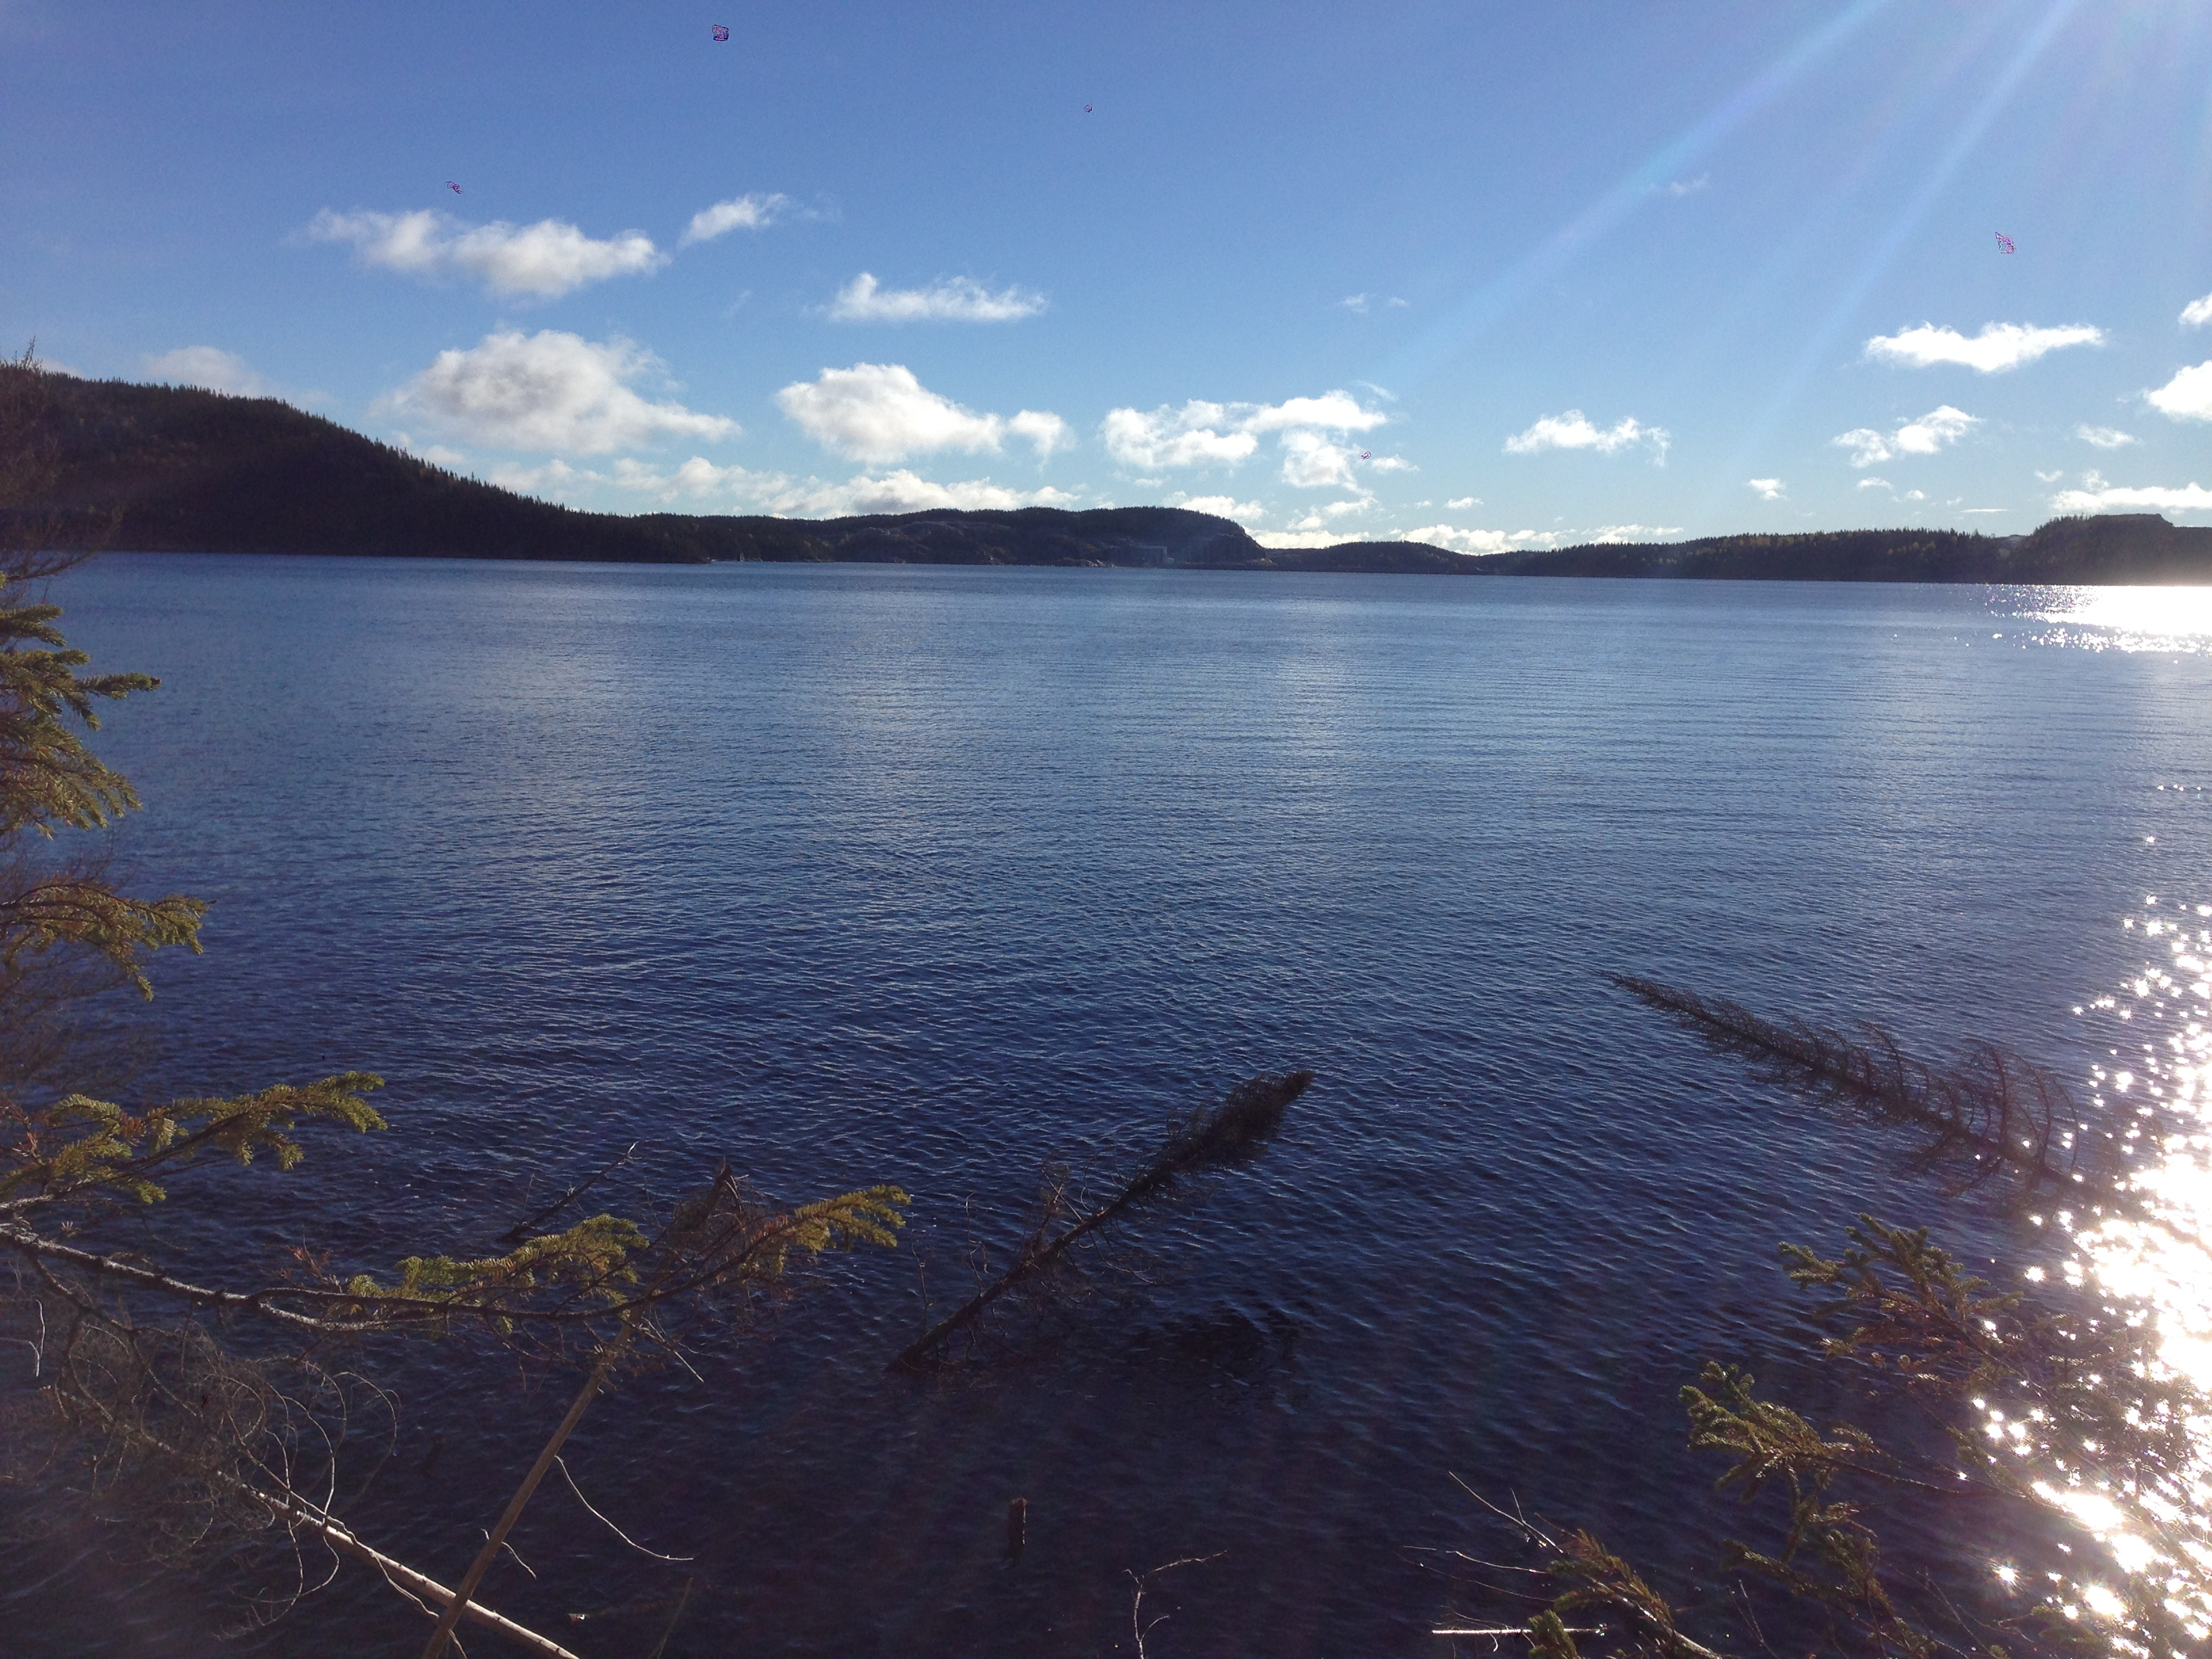
\includegraphics[height=2cm,width=\textwidth]{IMG_1923.JPG}}
\titlepage
\vskip.3cm
{
\includegraphics[scale=.3]{Logo-UL.png}}\hskip1cm
{
\includegraphics[scale=.3]{Image1.png}}\hskip1cm
{
\includegraphics[scale=.3]{Image2.png}}\hskip1cm
{
\includegraphics[scale=.3]{Image3.png}}

\end{frame}

\begin{frame}<beamer>\frametitle{Contents}
  \tableofcontents[sectionstyle=hide/hide,subsectionstyle=show/shaded/hide ]
\end{frame}

\section{Mise en contexte et Objectifs}
\begin{frame}{Mise en contexte et Objectifs}

\begin{adjustbox}{max totalsize={1.6\textwidth}{0.8\textheight},center}
\tikzset{every picture/.style={line width=0.7pt}} 
\begin{tikzpicture}[x=0.75pt,y=0.75pt,yscale=-1,xscale=1]
\draw (309,21) node  [align=left] {Évaporation nette = E (après mise en eau) - E(avant mise en eau)};
\pause
\draw (148,53) node  [align=left] {{\small \textbf{\textit{Indicateurs}}}};
\pause
\draw  [color={rgb, 255:red, 128; green, 128; blue, 128 }  ,draw opacity=1 ][dash pattern={on 4.5pt off 4.5pt}] (218.06,39.33) -- (533.06,39.33) -- (533.06,67.33) -- (218.06,67.33) -- cycle ;
\draw (288,53) node  [align=left] {(E$\displaystyle _{RES})$};
\draw (466,53) node  [align=left] {(E$\displaystyle _{RIV} +E_{FOR})$};
\pause
\draw  [color={rgb, 255:red, 238; green, 30; blue, 30 }  ,draw opacity=0.99 ][dash pattern={on 7.88pt off 4.5pt}][line width=3]  (29.06,39.53) -- (407,39.53) -- (407,67.33) -- (29.06,67.33) -- cycle ;
\draw (313,97) node  [align=left] {{\LARGE Modélisation} de l' évaporation sur le réservoir};
\draw (314,128) node [scale=0.9,color={rgb, 255:red, 0; green, 0; blue, 0 }  ,opacity=1 ] [align=left] {{\Large Modèle de lac 1D non couplé : \textit{\textbf{Canadian Small Lake Model}}}};
%Down Arrow [id:dp45351130193489064] 
\draw  [color={rgb, 255:red, 155; green, 155; blue, 155 }  ,draw opacity=1 ][dash pattern={on 4.5pt off 4.5pt}] (84.06,170.6) -- (194.31,170.6) -- (194.31,146) -- (414.81,146) -- (414.81,170.6) -- (525.06,170.6) -- (304.56,187) -- cycle ;

\draw    (156,190) -- (436,190) -- (436,220) -- (156,220) -- cycle  ;
\draw (296,205) node  [align=left] {{\Large Évaluer et valider le modèle }};
\pause
% Text Node
\draw (55,215) node [color={rgb, 255:red, 74; green, 144; blue, 226 }  ,opacity=1 ] [align=left] {\textit{\underline{Comment?}}};
%\draw    (367.06,220) -- (585.06,220) -- (585.06,242) -- (367.06,242) -- cycle  ;
\draw (476.06,231) node  [align=left] {\textbf{Implémenter par observation}};
%\draw    (78.5,222) -- (363.5,222) -- (363.5,244) -- (78.5,244) -- cycle  ;
\draw (150,231) node  [align=left] {\textbf{Comparer les sorties aux observations}};
\draw    (203,341) -- (409,341) -- (409,371) -- (203,371) -- cycle  ;

\pause
\draw (328,266) node [scale=1.44,color={rgb, 255:red, 227; green, 60; blue, 79 }  ,opacity=1 ] [align=left] {\textbf{Observations }};
\draw  [dash pattern={on 1.69pt off 2.76pt}][line width=1.5]  (131.06,262.2) .. controls (131.06,258.22) and (134.28,255) .. (138.26,255) -- (509.86,255) .. controls (513.83,255) and (517.06,258.22) .. (517.06,262.2) -- (517.06,283.8) .. controls (517.06,287.78) and (513.83,291) .. (509.86,291) -- (138.26,291) .. controls (134.28,291) and (131.06,287.78) .. (131.06,283.8) -- cycle ;

\draw (475,281) node [scale=1,color={rgb, 255:red, 0; green, 0; blue, 0 }  ,opacity=1 ] [align=left] {\textit{\textbf{Lac Piché}}};

\draw (195,280) node [scale=1,color={rgb, 255:red, 0; green, 0; blue, 0 }  ,opacity=1 ] [align=left] {\textbf{{\small Réservoir RO2}}};
\pause
\draw  [color={rgb, 255:red, 155; green, 155; blue, 155 }  ,draw opacity=1 ][dash pattern={on 4.5pt off 4.5pt}] (101.06,315.6) -- (211.31,315.6) -- (211.31,291) -- (431.81,291) -- (431.81,315.6) -- (542.06,315.6) -- (321.56,332) -- cycle ;
\draw (306,356) node  [align=left] {{\Large Améliorer le modèle }};
\pause
%\draw  [color={rgb, 255:red, 155; green, 155; blue, 155 }  ,draw opacity=1 ][dash pattern={on 4.5pt off 4.5pt}] (101.06,315.6) -- (211.31,315.6) -- (211.31,291) -- (431.81,291) -- (431.81,315.6) -- (542.06,315.6) -- (321.56,332) -- cycle ;
%Down Arrow [id:dp5013958201618147] 
\draw  [color={rgb, 255:red, 155; green, 155; blue, 155 }  ,draw opacity=1 ][dash pattern={on 4.5pt off 4.5pt}] (91.06,400.6) -- (201.31,400.6) -- (201.31,376) -- (421.81,376) -- (421.81,400.6) -- (532.06,400.6) -- (311.56,417) -- cycle ;
\draw (305,434) node  [align=left] {{\Large  \ Modèle de lac : \textbf{\textcolor[rgb]{0.87,0.2,0.12}{évalué, validé et amélioré}}}};
\draw    (138,453) -- (506,453) -- (506,483) -- (138,483) -- cycle  ;
\draw (322,468) node [scale=1.2] [align=left] {{\large Modéliser l'E sur RO1,RO2,RO3,RO4}};
\end{tikzpicture}
\end{adjustbox}
\end{frame}
\section{Matériel expérimental}
\subsection{Sites d'études : Complexe la Romaine}
\begin{frame}{Complexe la Romaine}
\begin{columns}
\column{0.5\textwidth}
\begin{figure}
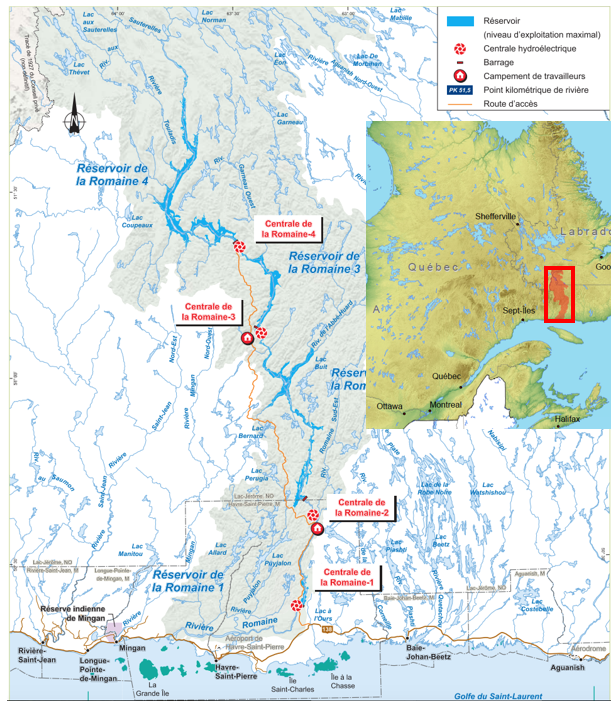
\includegraphics[scale=0.5]{projet.PNG}
\end{figure}
\column{0.5\textwidth}
\begin{enumerate}
\item Complexe hydroélectrique de la rivière Romaine
\item Côte-Nord à l’est du Québec
\item Bassin versant  14350 km$^2$ 
\item Quatre centrales alimentées par des réservoirs (RO1,RO2,RO3,RO4)
 \end{enumerate}
\end{columns}
\end{frame}

\begin{frame}{Réservoir de la Romaine 2}
\begin{columns}
\column{0.5\textwidth}
\begin{figure}
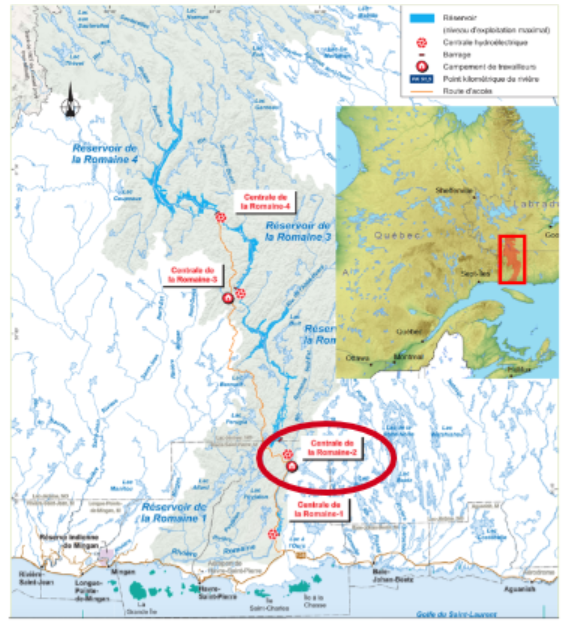
\includegraphics[scale=0.5]{ro2.png}
\end{figure}
\column{0.5\textwidth}
\begin{enumerate}
\item Superficie de 85 km$^2$ 
\item Mise en service en 2014, puissance de production de 640 MW
 \end{enumerate}
\end{columns}
\end{frame}

\subsection{Sites d'études : Lac Piché}
\begin{frame}{Lac Piché}
\begin{columns}
\column{0.5\textwidth}
\begin{figure}
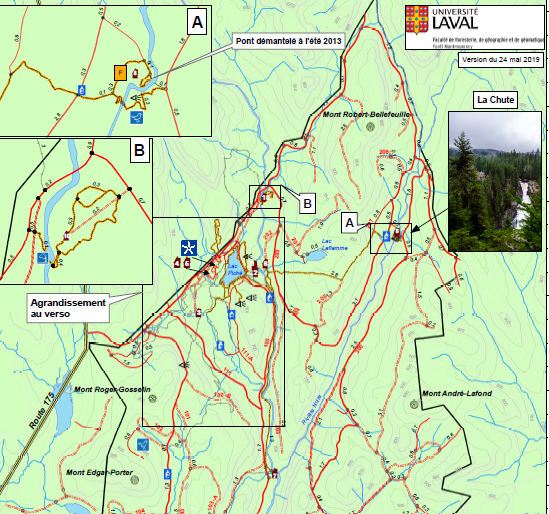
\includegraphics[scale=0.5]{FM.PNG}
\end{figure}
%\column{0.5\textwidth}
%\begin{itemize}
%\item La plus grande forêt d’enseignement et de recherche au monde de 397 km$^2$ 
%\end{itemize}
\column{0.5\textwidth}
\begin{figure}
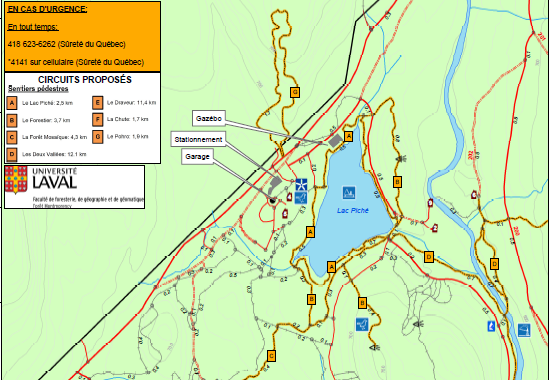
\includegraphics[scale=0.5]{LP.PNG}
\end{figure}
\end{columns}
\end{frame}
%\begin{frame}{Lac Piché}
%\begin{columns}

%\column{0.5\textwidth}
%\begin{enumerate}
%\item Superficie de 5 km$^2$ 
%\item Profondeur maximale de 5 m, régime d'eau non naturel.
% \end{enumerate}
%\end{columns}
%\end{frame}
\subsection{Bases de données : Réanalyses}
\begin{frame}{Compagne de mesure : Lac Piché}
    \begin{figure}
    \includegraphics<1>[scale=0.3]{rcs.PNG}
    \includegraphics<2>[scale=0.08]{camera_chasse.jpg}
    \includegraphics<3>[scale=0.08]{therm.jpg}
     \includegraphics<4>[scale=0.3]{glace.png}
     \includegraphics<5>[scale=0.3]{carotte.png}
    \caption{\only<1>{Variables métérologiques : station de mesure proche du lac}\only<2>{période gel/dégel}\only<3>{Chaine de thermistors}\only<4>{Suivi de l'épaisseur de glace et de neige}\only<5>{Caractérisation de la glace}}
\end{figure}
\end{frame}

\section{Outil de modélisation : Canadian Small Lake Model}
\subsection{CSLM : un modèle de lac}
\begin{frame}{\Large{C}\tiny{anadian} \Large{S}\tiny{mall} \Large{L}\tiny{ake} \Large{M}\tiny{odel}}
1D thermal model in absence of tubulence (energy budget at the surface)

\end{frame}

\subsection{Configuration du modèle : forçage métérologique}
\begin{frame}{Données de réanalyses : Réservoir la Romaine 2}
\begin{adjustbox}{max totalsize={1.2\textwidth}{1.2\textheight},center}
    \tikzset{every picture/.style={line width=0.75pt}} 
    \tikzset{every picture/.style={line width=0.75pt}}       
\begin{tikzpicture}[x=0.75pt,y=0.75pt,yscale=-1,xscale=1]
\draw (362.5,154.67) node  {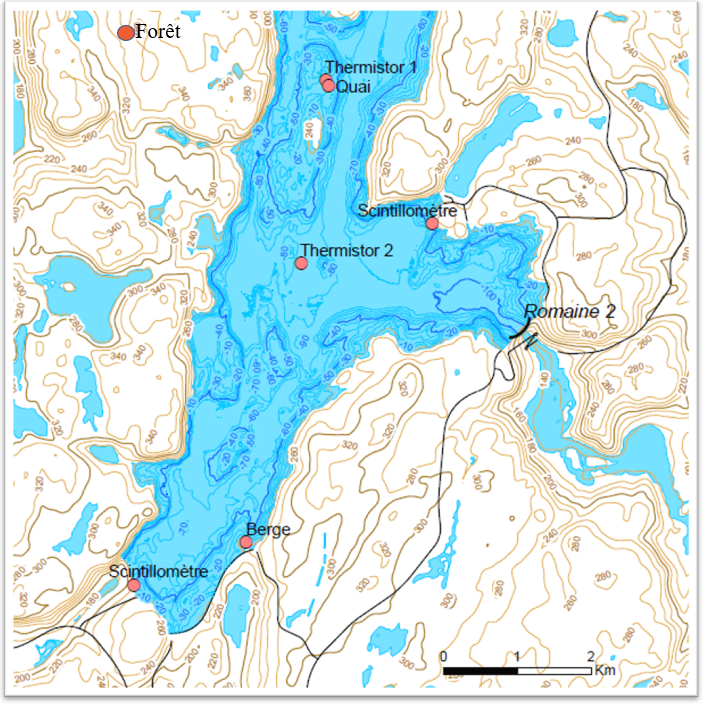
\includegraphics[width=241.5pt,height=200pt]{stations.PNG}};
\pause
\draw   (299,172.33) .. controls (299,168.93) and (301.57,166.17) .. (304.75,166.17) .. controls (307.93,166.17) and (310.5,168.93) .. (310.5,172.33) .. controls (310.5,175.74) and (307.93,178.5) .. (304.75,178.5) .. controls (301.57,178.5) and (299,175.74) .. (299,172.33) -- cycle ; \draw   (300.68,167.97) -- (308.82,176.69) ; \draw   (308.82,167.97) -- (300.68,176.69) ;
\draw    (199,172.33) .. controls (238.6,142.63) and (258.6,201.14) .. (297.81,173.21) ;
\draw [shift={(299,172.33)}, rotate = 503.13] [color={rgb, 255:red, 0; green, 0; blue, 0 }  ][line width=0.75]    (10.93,-3.29) .. controls (6.95,-1.4) and (3.31,-0.3) .. (0,0) .. controls (3.31,0.3) and (6.95,1.4) .. (10.93,3.29)   ;
\draw  [fill={rgb, 255:red, 255; green, 255; blue, 255 }  ,fill opacity=1 ] (98.9,132) -- (244.5,132) -- (244.5,179.52) .. controls (153.5,179.52) and (171.7,196.66) .. (98.9,185.57) -- cycle ; \draw  [fill={rgb, 255:red, 255; green, 255; blue, 255 }  ,fill opacity=1 ] (80.7,139.2) -- (226.3,139.2) -- (226.3,186.72) .. controls (135.3,186.72) and (153.5,203.86) .. (80.7,192.77) -- cycle ; \draw  [fill={rgb, 255:red, 255; green, 255; blue, 255 }  ,fill opacity=1 ] (62.5,146.4) -- (208.1,146.4) -- (208.1,193.92) .. controls (117.1,193.92) and (135.3,211.06) .. (62.5,199.97) -- cycle ;

% Text Node
\draw (133,174) node [scale=0.9,color={rgb, 255:red, 208; green, 2; blue, 27 }  ,opacity=1 ] [align=left] {{\fontfamily{ptm}\selectfont \textbf{\textcolor[rgb]{0,0,0}{Extraction ERA5 data }}}\\{\fontfamily{ptm}\selectfont \textbf{\textcolor[rgb]{0,0,0}{50.66, -63.21}}}};
\end{tikzpicture}
\end{adjustbox}
\end{frame}
\begin{frame}{ERA5 forcing data (moyenne inter-mensuelle 1981-2018)}

\end{frame}
\begin{frame}{Configuration du modèle : conditions intiales}

\begin{itemize}
\item<1->{\textbf{Profondeur adoptée}= 25 m, pas de sédiments au fond}
\item<2->{\textbf{Période de simulation}: du 01-01-1981 jusqu'au 31-12-2018 à pas de temps horaire}
\item<3->{\textbf{Période de chauffe}= 5 years (1981-1986)}
\item<4->{Fetch= 2000 m}
\item<5-> {\textbf{Caractéristiques optiques}: coefficient extinction  de l'eau= 2 m$^{-1}$}
\end{itemize}
\end{frame}

\section{Résultats préliminaires}
\begin{frame}{Profiles thermiques : CSLM vs Observations}
\end{frame}

\subsection{Différence lac-air températures}
\begin{frame}{Comparaison Tw et Ta}
\end{frame}
\subsection{Flux turbulents}
\begin{frame}{Profiles thermiques : CSLM vs Observations}
\end{frame}
\subsection{Flux radiatifs}
\subsection{Épaisseur de la glace}
\begin{frame}{Couche de glace}
\begin{minipage}{0.45\textwidth} % figure
\begin{figure}
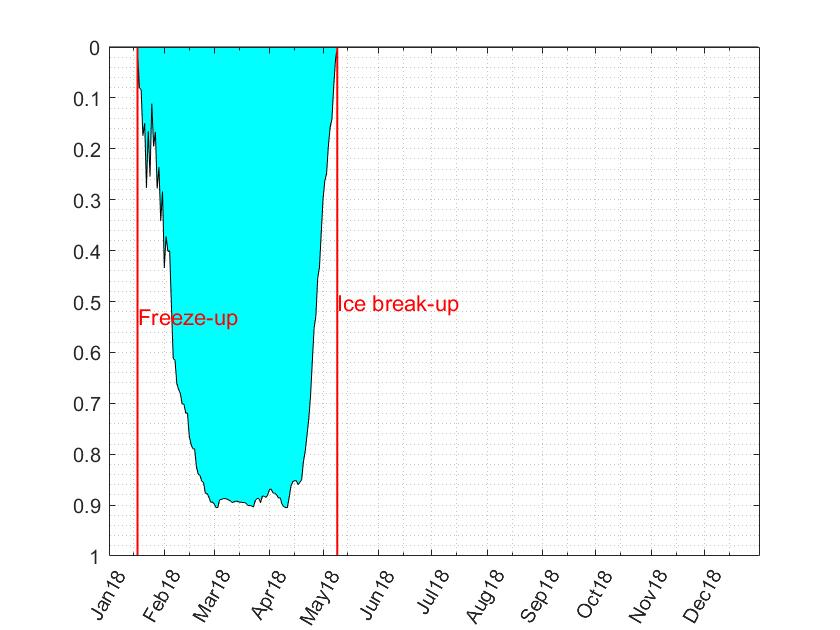
\includegraphics[scale=.25]{ICE2018.jpg}
\end{figure}
 \end{minipage}
\qquad
\begin{minipage}{5cm} % figure
\begin{figure}
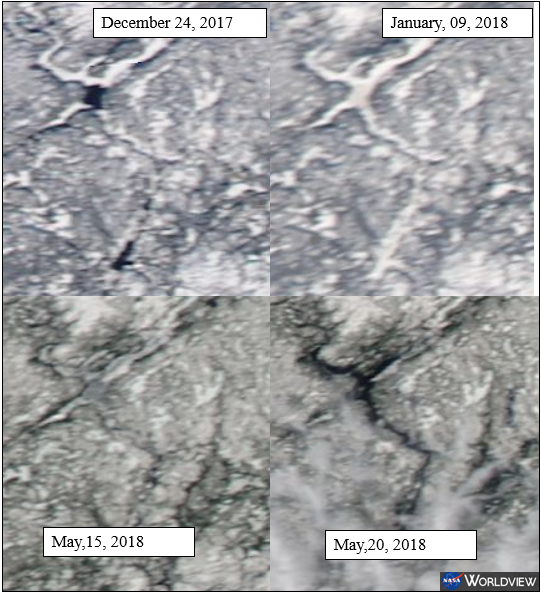
\includegraphics[scale=.5]{Ice_RO2.PNG}
\end{figure}
%\transduration<0-16>{0}
%\multiinclude[<+->][format=jpg, graphics={width=0.8\textwidth}]{ice}
 \end{minipage}
    \qquad
\begin{minipage}{7cm}
\begin{itemize}
\item<1->\parbox{\linewidth}{\only<1>{Maximum ice thickness: 85cm
}
\only<2>{Freeze-up: middle of january, begining of May: break-up (slow process)}
\only<3->{Simulated versus observed satellite imagery: delay of 8-11 days}}
\end{itemize}
\end{minipage}
\end{frame}
\section{Plan du futur travail}

\begin{frame}{}
  \centering \Huge
  \emph{Merci de votre attention}
\end{frame}
\end{document}
